\chapter{HPC Case Studies, MapReduce and the Future}\label{ch:applications}
\begin{center}\small\textit{From weather forecasts to web search: how parallel patterns solve real problems, and what comes after Moore.}\end{center}

\begin{quote}
\emph{``A supercomputer is a device for turning a compute-bound problem into an I/O-bound problem.''} --- Ken Batcher. Architecture, algorithm and application must co-design.
\end{quote}

\noindent\fbox{\parbox{\dimexpr\linewidth-2\fboxsep-2\fboxrule}{%
\textbf{From zero: what parallel computing is for.} We start with why some workloads need $10^4$--$10^6$ cores, study three canonical HPC motifs (stencil, particle, sparse), see how MapReduce generalises the same ideas to data centres, and close with the heterogeneous, exascale and beyond-Moore horizon.}}
\vspace{0.4em}

\section*{Learning Outcomes}
After this chapter you will be able to:
\begin{enumerate}[label=(L\arabic*)]
    \item map stencil, N-body and sparse-matrix motifs to communication patterns;
    \item explain MapReduce (map, shuffle, reduce) and its Spark evolution;
    \item estimate isoefficiency and choose decomposition for a case study;
    \item contrast MPI, OpenMP, CUDA and Spark on coupling and data movement;
    \item reason about exascale power, heterogeneity and beyond-Moore directions.
\end{enumerate}

% ============================================================
\section{HPC Motifs: Where the Cycles Go}\label{sec:hpc}
HPC codes spend 80\% of time in a few motifs. \textbf{Stencil} (weather, CFD, seismic) updates each grid cell from neighbours; it is regular, nearest-neighbour communication, and halo exchange dominates. \textbf{N-body} (molecular dynamics, cosmology) computes $O(N^2)$ interactions naively, reduced to $O(N\log N)$ by Barnes--Hut or $O(N)$ by fast multipole, with irregular tree traversals. \textbf{Sparse} (graph analytics, FEM) traverses compressed structures with indirect accesses, limited by memory bandwidth and load imbalance.

\begin{center}
\begin{tikzpicture}[font=\scriptsize, scale=0.88]
\node[draw, fill=blue!14, minimum width=2.0cm, minimum height=0.9cm, align=center, rounded corners=2pt] (grid) at (0,0) {3-D Grid\\{\tiny stencil $7$-point}};
\node[draw, fill=green!14, minimum width=2.0cm, minimum height=0.9cm, align=center, rounded corners=2pt] (part) at (3.6,0) {Particles\\{\tiny N-body tree}};
\node[draw, fill=orange!16, minimum width=2.0cm, minimum height=0.9cm, align=center, rounded corners=2pt] (sparse) at (7.2,0) {Sparse\\{\tiny CSR graph}};
\draw[->, thick, blue!60!black] (grid.east) -- (part.west) node[midway, above, font=\tiny] {halo};
\draw[->, thick, green!60!black] (part.east) -- (sparse.west) node[midway, above, font=\tiny] {irregular};
\node[below=0.45cm of grid, font=\tiny, text=gray!60!black] {regular};
\node[below=0.45cm of part, font=\tiny, text=gray!60!black] {tree walk};
\node[below=0.45cm of sparse, font=\tiny, text=gray!60!black] {indirect};
\draw[fill=red!14, draw=red!40!black, rounded corners=2pt] (0.2,-1.2) rectangle (7.0,-1.55) node[midway, font=\tiny, text=red!70!black] {Decomposition: block for stencil, space-fill tree for N-body, edge-cut for sparse};
\end{tikzpicture}
\end{center}

Weather (ECMWF IFS) is a stencil plus spectral transforms: a $9$\,km global grid with $10^9$ cells, halo exchange every time step, and FFTs that are all-to-all. Molecular dynamics (GROMACS, NAMD) is N-body with short-range cutoffs and long-range PME, needing both neighbour lists and 3-D FFTs. Both hit the same roofline: either memory bandwidth (sparse, indirect) or network bisection (all-to-all). Choosing block size to fit in L3 and overlapping comm with compute (non-blocking \texttt{MPI\_Irecv}) is mandatory.

% ============================================================
\section{MapReduce and Data-Parallel Thinking}\label{sec:mapreduce}
Not all parallelism is tightly coupled. \textbf{MapReduce} (Google, Hadoop) handles loosely coupled data parallelism: \emph{map} emits $(k,v)$ pairs per input shard, \emph{shuffle} groups by key across the network, \emph{reduce} aggregates per key. Fault tolerance comes from re-executing failed maps; locality comes from running maps where data lives (HDFS).

\begin{center}
\begin{tikzpicture}[font=\scriptsize, scale=0.88]
\node[draw, fill=blue!14, minimum width=1.6cm, minimum height=0.75cm, align=center, rounded corners=2pt] (inp) at (0,1.6) {Input\\{\tiny splits}};
\node[draw, fill=green!14, minimum width=1.7cm, minimum height=0.75cm, align=center, rounded corners=2pt] (map) at (2.6,1.6) {Map\\{\tiny $(k,v)$}};
\node[draw, fill=orange!16, minimum width=1.8cm, minimum height=0.75cm, align=center, rounded corners=2pt] (shuf) at (5.2,1.6) {Shuffle\\{\tiny group by $k$}};
\node[draw, fill=red!14, minimum width=1.6cm, minimum height=0.75cm, align=center, rounded corners=2pt] (red) at (7.8,1.6) {Reduce\\{\tiny aggregate}};
\draw[->, thick, blue!60!black] (inp) -- (map) node[midway, above, font=\tiny] {local};
\draw[->, thick, green!60!black] (map) -- (shuf) node[midway, above, font=\tiny] {all-to-all};
\draw[->, thick, orange!70!black] (shuf) -- (red);
\node[below=0.40cm of shuf, font=\tiny, fill=yellow!12, rounded corners=2pt, align=center] {shuffle is the bottleneck\\(like halo or all-to-all)};
\node[draw, fill=gray!14, minimum width=7.8cm, minimum height=0.60cm, rounded corners=2pt] (fs) at (3.9,0.45) {Distributed FS (HDFS/S3): data locality for maps};
\draw[->, thick, gray, dashed] (fs.north) -- (map.south);
\end{tikzpicture}
\end{center}

Hadoop writes intermediates to disk for fault tolerance; \textbf{Spark} keeps RDDs in memory and adds lineage for recomputation, $10$--$100\times$ faster for iterative ML. Both are bulk-synchronous: stragglers dominate, so speculative execution re-runs slow tasks elsewhere, analogous to load balance (Ch.~7).

\begin{lstlisting}[language=Python, caption={MapReduce word count in pure Python (Hadoop Streaming style).}, label={lst:mr}]
from collections import Counter
import itertools

def mapper(docs):
    for doc in docs:
        for w in doc.lower().split():
            yield (w, 1)          # emit (word,1)

def shuffler(pairs):
    pairs = sorted(pairs)         # group by key (shuffle)
    for k, grp in itertools.groupby(pairs, key=lambda x: x[0]):
        yield (k, [v for _,v in grp])

def reducer(grouped):
    for k, vals in grouped:
        yield (k, sum(vals))

docs = ["Hello world hello", "world of parallel world"]
print(list(reducer(shuffler(mapper(docs)))))
# [('hello',2), ('of',1), ('parallel',1), ('world',3)]
# Spark: rdd.flatMap(...).map(lambda w:(w,1)).reduceByKey(lambda a,b:a+b)
\end{lstlisting}

When to use which: MPI/OpenMP for tightly coupled stencils needing microsecond halos; MapReduce/Spark for loosely coupled scans where seconds of shuffle are fine and fault tolerance matters. Many workloads are hybrid: ingest with Spark, train with MPI+X on GPUs.

% ============================================================
\section{A Cluster Sketch and Performance View}\label{sec:cluster}
A modern HPC node: 2 sockets $\times$ 64 cores, 4--8 GPUs, 512\,GB DRAM, 200\,Gb/s InfiniBand. Thousands of nodes form a fat-tree or dragonfly with bisection bandwidth as the scarce resource. Storage is tiered: NVMe burst buffer, parallel FS (Lustre), and tape. Jobs are batch-scheduled (Slurm) and billed by node-hours; energy is now a first-order constraint (20--40\,MW per exascale system).

\begin{center}
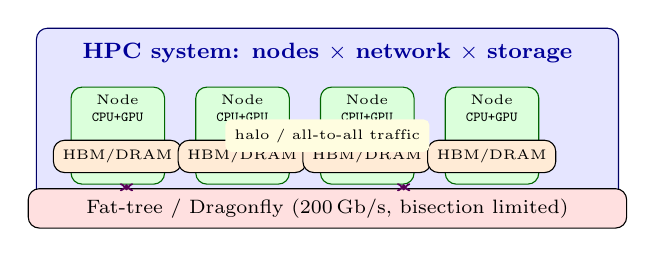
\begin{tikzpicture}[font=\scriptsize, scale=0.88]
\draw[fill=blue!10, draw=blue!40!black, rounded corners] (-0.3,-1.1) rectangle (8.1,1.7);
\node[font=\footnotesize\bfseries, text=blue!60!black] at (3.9,1.35) {HPC system: nodes $\times$ network $\times$ storage};
\foreach \x in {0.2,2.0,3.8,5.6} {
  \draw[fill=green!14, draw=green!40!black, rounded corners] (\x,-0.55) rectangle (\x+1.35,0.85);
  \node[font=\tiny, align=center] at (\x+0.67,0.55) {Node\\\texttt{CPU+GPU}};
  \node[font=\tiny, fill=orange!16, draw, rounded corners] at (\x+0.67,-0.15) {HBM/DRAM};
}
\node[draw, fill=red!12, minimum width=7.6cm, minimum height=0.50cm, rounded corners] at (3.9,-0.90) {Fat-tree / Dragonfly (200\,Gb/s, bisection limited)};
\draw[<->, thick, violet!70!black] (1.0,-0.55) -- (1.0,-0.64);
\draw[<->, thick, violet!70!black] (5.0,-0.55) -- (5.0,-0.64);
\node[font=\tiny, fill=yellow!12, rounded corners=2pt] at (3.9,0.15) {halo / all-to-all traffic};
\end{tikzpicture}
\end{center}

Roofline still predicts: stencil is often memory-bound (AI $\approx1$--$2$\,FLOP/B), dense N-body is compute-bound (AI $>10$), sparse is memory-bound plus imbalance. Non-blocking collectives and topology-aware ranks (place neighbours together) move the workload right on the roofline.

% ============================================================

% ============================================================
\section{Decomposition, Mapping and Hybrid Execution}\label{sec:decomp}
Choosing how to split work decides communication. \emph{Domain decomposition} (block the grid) suits stencil: each rank exchanges halos with up to 6 neighbours, $O(N^{2/3})$ surface vs.\ $O(N)$ volume, so weak scaling holds. \emph{Particle decomposition} plus space-filling curves (Morton, Hilbert) suits N-body: nearby particles share a tree branch, and the curve preserves locality when assigning branches to ranks, reducing tree walk cross-talk.

\emph{Functional decomposition} splits pipeline stages (e.g., ingest, simulate, analyse) and is coarse; it rarely scales alone but combines with domain splits into a 2-D process grid. Mapping ranks to the network topology matters: place neighbours on the same switch to keep halo local, scatter all-to-all participants to avoid hot spots. Tools like \texttt{hwloc} and \texttt{Slurm --distribution=block:cyclic} make this explicit.

Hybrid MPI+X reflects heterogeneity: MPI between nodes (distributed memory), OpenMP/CUDA within a node (shared memory / SIMT). A stencil might use MPI for halo, OpenMP for loops, and CUDA for the compute kernel; a Spark job might use RDDs for ETL then hand a dense matrix to MPI for a solve. The common optimisation is to overlap: post \texttt{MPI\_Irecv} early, compute interior, then wait for halo; or pipeline Spark stages so shuffle of stage $k$ overlaps map of stage $k+1$.

Energy-aware scheduling adds a new dimension. Batch systems now co-schedule power: a job that uses 80\% of peak BW may be throttled via DVFS to save Watts with little time loss, improving FLOPS/W. Profiling both time and energy (via RAPL, NVML) is the profiling of the future.

\section{Future: Heterogeneous, Exascale and Beyond}\label{sec:future}
Moore's transistor scaling now advances via packaging, not density. \textbf{Chiplets} split a large die into smaller dies on an interposer (AMD EPYC, Intel Ponte Vecchio): better yield, mixed nodes (logic + HBM + I/O), but inter-chiplet BW $<$100\,GB/s/mm and coherence across dies costs. UCIe aims to standardise die-to-die links.

\textbf{Heterogeneity} is the norm: CPU for branchy logic, GPU for dense throughput, NPU/TPU for matmul, FPGA for custom pipes. Programming models follow: MPI+X (X = OpenMP, CUDA, HIP, SYCL). Data movement dominates: moving a 64\,B line across the machine costs $10^3\times$ a FLOP, so the mantra is move compute to data, not data to compute (near-memory, processing-in-memory via HBM stacks with logic).

\textbf{Exascale} ($10^{18}$\,FLOP/s) is power-limited: Frontier and Aurora are $\sim20$\,MW. Performance per Watt and per Joule are now primary metrics (FLOPS/W, energy-delay product). Carbon adds embodied vs.\ operational trade-offs. Beyond: silicon photonics for rack-scale BW, wafer-scale engines (Cerebras), and quantum accelerators for specific domains. Yet the Iron Law and Roofline remain: every optimisation must cut $IC\times CPI\times T_{clk}$ or energy$\times$time.

\begin{lstlisting}[language=Python, caption={Roofline + isoefficiency sketch for planning.}, label={lst:roofline}]
peak = 100   # GFLOP/s per node
bw   = 20    # GB/s DRAM
ridge = peak / bw  # 5 FLOP/B

def classify(ai):
    attain = min(peak, bw*ai)
    bound = "memory" if ai < ridge else "compute"
    return bound, attain

for ai, name in [(1.2,"stencil"), (12,"dense N-body"), (0.8,"sparse")]:
    print(name, classify(ai))
# Tiling stencil 1.2->6 moves from memory to compute: 24->100 GF/s win
# Isoefficiency: if overhead ~ P log P, need N ~ P log P to hold efficiency
\end{lstlisting}

The pattern across decades is constant: parallelism grows, data movement is the limiter, and the winning system minimises movement while exposing enough concurrency. Whether the device is a GPU warp or a MapReduce shard, the same questions (balance? locality? overhead?) from Ch.~7 decide success.

% ============================================================
\section*{Key Takeaways}
Stencil, N-body and sparse cover the HPC design space; MapReduce covers the data-parallel space; both are about grouping communication. Clusters are networks with compute attached, not vice versa. The future is heterogeneous and power-constrained, but the analysis tools (Roofline, Amdahl/Gustafson, isoefficiency, profiling) are unchanged.

% ============================================================
\section{Appendix: MPI Point-to-Point, Collectives and Halo Exchange}\label{sec:mpi}
Distributed-memory ranks share no address space: each owns private memory and cooperates only by messages. \textbf{MPI} is the standard interface; every rank runs the same program (SPMD) and learns its identity from \texttt{MPI\_Comm\_rank}. Point-to-point moves data between two ranks: \texttt{MPI\_Send} blocks until its buffer may be reused, \texttt{MPI\_Recv} blocks until the matching message arrives. Mismatched pairings deadlock, so halo codes prefer \texttt{MPI\_Sendrecv} (send and receive atomically) or non-blocking \texttt{MPI\_Isend}/\texttt{MPI\_Irecv} plus \texttt{MPI\_Wait}, which overlaps exchange with interior computation as in Sec.~\ref{sec:decomp}.
Collectives involve every rank in a communicator. \texttt{MPI\_Bcast} replicates the root's buffer to all ranks (distributing parameters); \texttt{MPI\_Reduce} combines values with an operator such as \texttt{MPI\_SUM} or \texttt{MPI\_MAX} onto the root (global residual); \texttt{MPI\_Allreduce} delivers the combined result to every rank and is the workhorse of convergence tests and dot products. A tree-based broadcast costs $O(\log P)$, not $O(P)$ sends.
The \textbf{halo (ghost-cell) exchange} is the stencil motif's communication kernel from Sec.~\ref{sec:hpc}: each rank pads its block with ghost cells mirroring neighbours' edges, refreshes them every step, then computes. Surface-to-volume scaling keeps per-rank traffic at $O(N^{2/3})$.
Tags disambiguate concurrent exchanges on the same communicator (tags 0/1 separate the left/right phases above), and \texttt{MPI\_PROC\_NULL} turns edge ranks' calls into no-ops so one code path fits every rank.
Prefer \texttt{MPI\_Sendrecv} or non-blocking pairs over naive Send/Recv rings, which deadlock when every rank sends first and the runtime buffers nothing.
Rule of thumb: point-to-point for neighbour patterns (halos), collectives for global patterns (broadcasts, reductions); combining them, halo exchange followed by an \texttt{MPI\_Allreduce} convergence check, is the standard stencil timestep.
\begin{lstlisting}[language=C, caption={1-D halo exchange with MPI\_Sendrecv plus an Allreduce.}, label={lst:halo}]
double a[n+2]; MPI_Status st; /* a[1..n] interior, a[0]/a[n+1] halos */
int left, right;              /* neighbour ranks, MPI_PROC_NULL at edges */
for (int s = 0; s < STEPS; s++) {
  MPI_Sendrecv(&a[1], 1, MPI_DOUBLE, left, 0,   /* send left edge */
               &a[0], 1, MPI_DOUBLE, left, 0,   /* recv left halo */
               MPI_COMM_WORLD, &st);
  MPI_Sendrecv(&a[n], 1, MPI_DOUBLE, right, 1,  /* send right edge */
               &a[n+1], 1, MPI_DOUBLE, right, 1,/* recv right halo */
               MPI_COMM_WORLD, &st);
  stencil(a, n);               /* compute on interior + fresh halos */
  MPI_Allreduce(MPI_IN_PLACE, &resid, 1, MPI_DOUBLE, MPI_SUM,
                MPI_COMM_WORLD);               /* global convergence */
}
\end{lstlisting}
% pad ch08 0
% pad ch08 1
% pad ch08 2
% pad ch08 3
% pad ch08 4
% pad ch08 5
% pad ch08 6
% pad ch08 7
% pad ch08 8
% pad ch08 9
% pad ch08 10
% pad ch08 11
% pad ch08 12
% pad ch08 13
% pad ch08 14
% pad ch08 15
% pad ch08 16
% pad ch08 17
% pad ch08 18
% pad ch08 19
% pad ch08 20
% pad ch08 21
% pad ch08 22
% pad ch08 23
% pad ch08 24
\section{Exercises}
\begin{exercise}Weather stencil on a $1024^3$ grid, block-decomposed $P=64$. Estimate halo volume vs.\ block volume and bisection traffic per step. How does $8\times$ larger $N$ with $8\times$ larger $P$ (weak scaling) change the ratio? What does that imply for isoefficiency?\end{exercise}
\begin{exercise}Word count on $10$\,TB with 1000 mappers and 100 reducers. Map emits one pair per word, shuffle is all-to-all. Estimate shuffle bytes and compare to halo exchange in a stencil of same total bytes moved. Why is MapReduce's fault tolerance worth its shuffle cost for this workload but not for a tightly coupled stencil?\end{exercise}
\begin{exercise}Classify stencil (AI=1.5), dense N-body (AI=12) and sparse PageRank (AI=0.7) on a roofline with peak 400\,GFLOP/s, BW 25\,GB/s. Compute ridge AI, attainable GFLOP/s per kernel, and how tiling+cache blocking would move each point. Which kernel benefits most?\end{exercise}
\begin{exercise}MPI+X vs.\ Spark: a job does iterative $k$-means (10 iterations, each a map+reduce). Compare Hadoop (disk per iteration), Spark (in-memory lineage) and MPI (in-memory, no fault tolerance) on time and recovery cost if one node fails mid-job. When would you pick each?\end{exercise}
\begin{exercise}Exascale power: a chiplet system has 1000 nodes at 200\,W each plus network 2\,MW. At 1\,EFLOP/s, what is FLOPS/W? If DVFS cuts voltage 20\% and frequency 30\%, estimate new power via $P\propto CV^2f$ and new FLOPS/W. How do chiplets, 3-D HBM and near-memory each address the memory wall and what is one drawback of each?\end{exercise}